\documentclass[tikz,border=8pt]{standalone}
% Shared look for every TikZ diagram. Load with \input{../../tools/tikz-style.tex}
\usepackage[T1]{fontenc}
\usepackage{lmodern}
\renewcommand{\sfdefault}{lmr}  % diagrams use the same serif as the text
\usetikzlibrary{arrows.meta, positioning, shapes.geometric, calc, fit, backgrounds}
\definecolor{cblue}{HTML}{4C78A8}
\definecolor{corange}{HTML}{F58518}
\definecolor{cgreen}{HTML}{54A24B}
\definecolor{cred}{HTML}{E45756}
\definecolor{cpurple}{HTML}{B279A2}
\definecolor{cgrey}{HTML}{6B6B6B}
\tikzset{
  every picture/.style={font=\sffamily, line width=1.2pt},
  box/.style={draw=#1, fill=#1!12, rounded corners=4pt, align=center, inner sep=7pt, minimum height=1.1cm},
  box/.default=cgrey,
  arrow/.style={-{Stealth[length=3mm]}, draw=cgrey, line width=1.4pt},
  title/.style={font=\sffamily\bfseries\Large},
  note/.style={font=\sffamily\small, text=cgrey, align=center},
}
\AtBeginDocument{\hyphenpenalty=10000 \exhyphenpenalty=10000}

% Expected range and bearing of the pink pole (4.4, 3.8) from a pose (2, 2, theta). dx = 2.4, dy = 1.8:
% range sqrt(2.4^2 + 1.8^2) = 3.0; direction atan2(1.8, 2.4) = 36.87 deg; bearing = direction - heading.
% Drawn with heading theta = 15 deg to show the subtraction (the Note's pose A has theta = 0).
\begin{document}
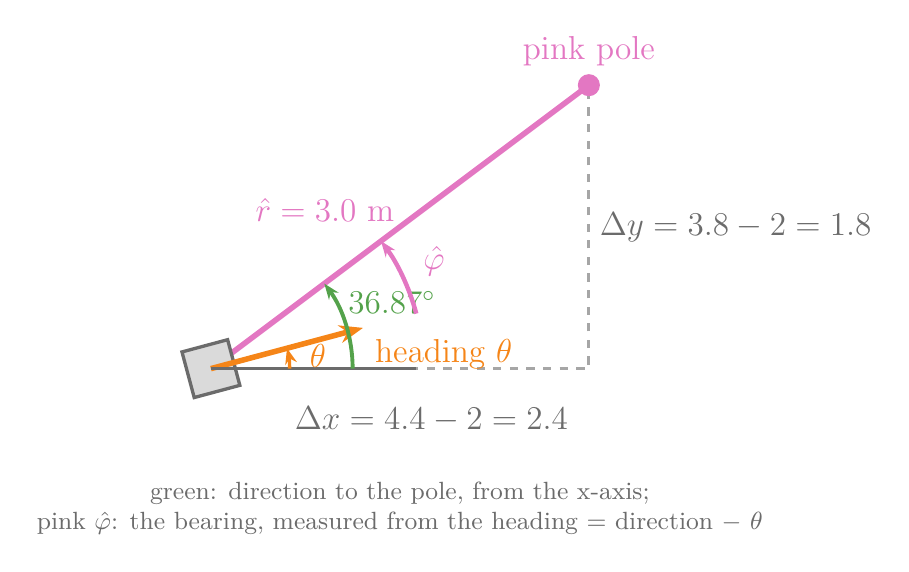
\begin{tikzpicture}[scale=2.0, every node/.append style={font=\large}]
  \definecolor{cpink}{HTML}{E377C2}
  \draw[cgrey!60, dashed, line width=1pt] (2,2) -- (4.4,2) -- (4.4,3.8);
  \node[below=10pt, cgrey] at (3.4,2) {$\Delta x = 4.4 - 2 = 2.4$};
  \node[right, cgrey] at (4.4,2.9) {$\Delta y = 3.8 - 2 = 1.8$};
  \draw[cpink, line width=2pt] (2,2) -- (4.4,3.8) node[midway, above left, fill=white, inner sep=1pt] {$\hat r = 3.0$ m};
  \fill[cpink] (4.4,3.8) circle (0.07);
  \node[cpink, above] at (4.4,3.85) {pink pole};
  \draw[cgrey, fill=cgrey!25, rotate around={15:(2,2)}] (1.85,1.85) rectangle (2.15,2.15);
  \draw[-{Stealth[length=3mm]}, corange, line width=2pt] (2,2) -- ++(15:1.0) node[below right] {heading $\theta$};
  \draw[cgrey, line width=1pt] (2,2) -- (3.3,2);
  \draw[cgreen, line width=1.4pt, -{Stealth[length=2mm]}] (2.9,2) arc (0:36.87:0.9);
  \node[cgreen] at (3.15,2.42) {$36.87^\circ$};
  \draw[corange, line width=1.2pt, -{Stealth[length=2mm]}] (2.5,2) arc (0:15:0.5);
  \node[corange] at (2.68,2.08) {$\theta$};
  \draw[cpink, line width=1.6pt, -{Stealth[length=2mm]}] ($(2,2)+(15:1.35)$) arc (15:36.87:1.35);
  \node[cpink, right] at ($(2,2)+(28:1.45)$) {$\hat\varphi$};
  \node[note, anchor=north, align=center] at (3.2,1.35) {green: direction to the pole, from the x-axis;\\ pink $\hat\varphi$: the bearing, measured from the heading $=$ direction $-$ $\theta$};
\end{tikzpicture}
\end{document}
